\documentclass[a4paper, 10pt, ]{article}

\usepackage[slovak]{babel}





\usepackage[utf8]{inputenc}
\usepackage[T1]{fontenc}

\usepackage[left=4cm,
			right=4cm,
            % left=2.5cm,
			% right=5.5cm,
			top=2.1cm,
			bottom=2.6cm,
			footskip=7.5mm,
			% twoside,
			marginparwidth=3.0cm,
			%showframe,
			]{geometry}

\usepackage{graphicx}
\usepackage[dvipsnames]{xcolor}
% https://en.wikibooks.org/wiki/LaTeX/Colors


% ------------------------------

\usepackage{lmodern}

\usepackage[tt={oldstyle=false,proportional=true,monowidth}]{cfr-lm}

% ------------------------------

\usepackage{amsmath}
\usepackage{amssymb}
\usepackage{amsthm}

\usepackage{booktabs}
\usepackage{multirow}
\usepackage{array}
\usepackage{dcolumn}


\usepackage[singlelinecheck=true]{subfig}


% ------------------------------


\def\naT{\mathsf{T}}

\hyphenpenalty=6000
\tolerance=1000




% ------------------------------


\makeatletter

	\def\@seccntformat#1{\protect\makebox[0pt][r]{\csname the#1\endcsname\hspace{4mm}}}

	\def\cleardoublepage{\clearpage\if@twoside \ifodd\c@page\else
	\hbox{}
	\vspace*{\fill}
	\begin{center}
	\phantom{}
	\end{center}
	\vspace{\fill}
	\thispagestyle{empty}
	\newpage
	\if@twocolumn\hbox{}\newpage\fi\fi\fi}

	\newcommand\figcaption{\def\@captype{figure}\caption}
	\newcommand\tabcaption{\def\@captype{table}\caption}

\makeatother


% ------------------------------




\usepackage{fancyhdr}
\fancypagestyle{plain}{%
\fancyhf{} % clear all header and footer fields
\fancyfoot[C]{\sffamily {\bfseries \thepage}\ | {\scriptsize\oznacenieCasti}}
\renewcommand{\headrulewidth}{0pt}
\renewcommand{\footrulewidth}{0pt}}
\pagestyle{plain}


% ------------------------------


\usepackage{titlesec}
\titleformat{\paragraph}[hang]{\sffamily  \bfseries}{}{0pt}{}
\titlespacing*{\paragraph}{0mm}{3mm}{1mm}
\titlespacing*{\subparagraph}{0mm}{3mm}{1mm}

\titleformat*{\section}{\sffamily\Large\bfseries}
\titleformat*{\subsection}{\sffamily\large\bfseries}
\titleformat*{\subsubsection}{\sffamily\normalsize\bfseries}






% ------------------------------

\PassOptionsToPackage{hyphens}{url}
\usepackage[pdfauthor={},
			pdftitle={},
			pdfsubject={},
			pdfkeywords={},
			% hidelinks,
			colorlinks=false,
			breaklinks,
			]{hyperref}


% ------------------------------


\graphicspath{%
{../fig_standalone/}%
{../../PY/fig/}%
{../../PY/jupynotex/fig/}%
{../../ML/fig/}%
{./fig/}%
}



% ------------------------------

\usepackage{enumitem}

\usepackage{lettrine}

% ------------------------------


\usepackage{microtype}


% ------------------------------

\usepackage[titles]{tocloft}

\setlength{\cftsecindent}{-12mm}
\setlength{\cftsecnumwidth}{12mm}
\renewcommand{\cftsecpresnum}{\hfill}
\renewcommand{\cftsecaftersnum}{\hspace{4mm}}

\setlength{\cftsubsecindent}{-12mm}
\setlength{\cftsubsecnumwidth}{16mm} % 12 + 4
\renewcommand{\cftsubsecpresnum}{\hfill}
\renewcommand{\cftsubsecaftersnum}{\hspace{8mm}} % 4 + 4 mm

\setlength{\cftsubsubsecindent}{-12mm}
\setlength{\cftsubsubsecnumwidth}{20mm} % 12 + 4 + 4
\renewcommand{\cftsubsubsecpresnum}{\hfill}
\renewcommand{\cftsubsubsecaftersnum}{\hspace{12mm}} % 4 + 4 + 4 mm

\renewcommand{\cftsecpagefont}{\lstyle \bfseries}
\renewcommand{\cftsubsecpagefont}{\lstyle}
\renewcommand{\cftsubsubsecpagefont}{\lstyle}



\setlength{\cftparaindent}{-16mm}
\setlength{\cftparanumwidth}{28mm} % 16 + 4 + 4 + 4
\renewcommand{\cftparapresnum}{\hfill}
\renewcommand{\cftparaaftersnum}{\hspace{16mm}} % 4 + 4 + 4 + 4 mm








% ------------------------------

\usepackage{listings}



\renewcommand{\lstlistingname}{Výpis kódu}
\renewcommand{\lstlistlistingname}{Výpisy kódu}




%New colors defined below
\definecolor{codegreen}{rgb}{0,0.6,0}
\definecolor{codegray}{rgb}{0.5,0.5,0.5}
\definecolor{codepurple}{rgb}{0.58,0,0.82}
\definecolor{backcolour}{rgb}{0.95,0.95,0.95}

%Code listing style named "mystyle"
\lstdefinestyle{mystyle}{
  backgroundcolor=\color{backcolour},
  commentstyle=\fontfamily{lmtt}\fontsize{8.5pt}{8.75pt}\selectfont\color{codegreen},
  keywordstyle=\fontfamily{lmtt}\fontsize{8.5pt}{8.75pt}\selectfont\bfseries\color{Blue},
  stringstyle=\fontfamily{lmtt}\fontsize{8.5pt}{8.75pt}\selectfont\color{codepurple},
  basicstyle=\fontfamily{lmtt}\fontsize{8.5pt}{8.75pt}\selectfont,
  breakatwhitespace=false,
  breaklines=true,
  captionpos=t,
  keepspaces=true,
  numbers=left,
  numbersep=4mm,
  numberstyle=\fontfamily{lmtt}\fontsize{8.5pt}{8.75pt}\selectfont\color{lightgray},
  showspaces=false,
  showstringspaces=false,
  showtabs=false,
  tabsize=2,
  % xleftmargin=10pt,
  framesep=10pt,
  language=Python,
  escapechar=|,
}


\lstset{
    inputencoding=utf8,
    extendedchars=true,
    literate=%
    {á}{{\'a}}1
    {č}{{\v{c}}}1
    {ď}{{\v{d}}}1
    {é}{{\'e}}1
    {ě}{{\v{e}}}1
    {í}{{\'i}}1
    {ň}{{\v{n}}}1
    {ó}{{\'o}}1
    {ř}{{\v{r}}}1
    {š}{{\v{s}}}1
    {ť}{{\v{t}}}1
    {ú}{{\'u}}1
    {ů}{{\r{u}}}1
    {ý}{{\'y}}1
    {ž}{{\v{z}}}1
    {Á}{{\'A}}1
    {Č}{{\v{C}}}1
    {Ď}{{\v{D}}}1
    {É}{{\'E}}1
    {Ě}{{\v{E}}}1
    {Í}{{\'I}}1
    {Ň}{{\v{N}}}1
    {Ó}{{\'O}}1
    {Ř}{{\v{R}}}1
    {Š}{{\v{S}}}1
    {Ť}{{\v{T}}}1
    {Ú}{{\'U}}1
    {Ů}{{\r{U}}}1
    {Ý}{{\'Y}}1
    {Ž}{{\v{Z}}}1
    {ô}{{\^{o}}}1
}


% ------------------------------


\usepackage{caption}

\DeclareCaptionFormat{odsadene}{\protect\makebox[0pt][r]{#1#2\hspace{4mm}}#3\par}
\DeclareCaptionLabelSeparator{lendvojbodka}{:}
% \DeclareCaptionFont{lightgray}{\color{lightgray}}
\DeclareCaptionFont{lightgray}{\fontfamily{lmtt}\fontsize{8.5pt}{8.75pt}\selectfont\color{lightgray}}

\captionsetup[lstlisting]{format=odsadene, labelsep=lendvojbodka, justification=raggedright, singlelinecheck=false, labelfont={sf, lightgray},}


% ------------------------------





% ------------------------------

\usepackage[backend=biber,
            style=numeric,
            sorting=none,
            ]{biblatex}
\DeclareSourcemap{
    \maps[datatype=bibtex]{
        \map{
        \step[fieldset=note, null]
        }
        \map{
        \step[fieldset=file, null]
        }        
        % \map{
        % \step[fieldset=url, null]        
        % }
        \map{
        \step[fieldset=eprint, null]
        }
    }
}


\addbibresource{E:/_CurrentContent/01_work_repo/bibLaTeXDB/bibLaTeXDB.bib} % nonpublic data





\def\oznacenieCasti{MRS01 - ZS2024}





\begin{document}


\lstset{%
style=mystyle,
rangebeginprefix=\#\#\#\ cellB\ ,%
rangebeginsuffix=\ \#\#\#,%
rangeendprefix=\#\#\#\ cellE\ ,%
rangeendsuffix=\ \#\#\#,%
includerangemarker=false,
}






\fontsize{12pt}{22pt}\selectfont

\centerline{\textsf{Modelovanie a riadenie systémov} \hfill \textsf{\oznacenieCasti}}

\fontsize{18pt}{22pt}\selectfont





\begin{flushleft}
	\textbf{\textsf{Cvičenie úvodné}}
\end{flushleft}






\normalsize

\bigskip

{\hypersetup{hidelinks}

\tableofcontents

}

\bigskip

\vspace{18pt}



\noindent
\lettrine[lines=3, nindent=0pt]{C}{ieľom} úvodného cvičenia je poskytnúť podnety k pojmu \emph{systém} z hľadiska predmetu Modelovanie a riadenie systémov. Materiál je zostavený tak, že študentstvo by sa ním malo vedieť zaoberať bez potreby predchádzajúcej prednášky. Je tým ošetrený prípad keď je v rámci týždňa nejaký termín cvičení skôr ako termín prednášky.

\bigskip

\noindent
Nasledujúce dva konkrétne príklady je možné využiť na úvodnú diskusiu k~nasledujúcim pojmom a témam:

\begin{itemize}[leftmargin=0pt, labelsep=1mm, itemsep=-4pt, topsep=0pt, ]
    \item Systém -- má výstup a vstup (môže mať len výstup\ldots)
    \item Signál. Na tomto predmete sa signál značí v princípe ako funkcia času, ako v čase premenlivá hodnota veličiny, teda napr. $y(t)$.
    \item Dynamický systém
    \item Systém, ktorého dynamiku nie je potrebné uvažovať.
    \item Rovnica ako nástroj pre matematický opis systému.
    \item Diferenciálna rovnica -- matematický opis dynamického systému.
\end{itemize}








\section{Úlohy}



\begin{enumerate}[leftmargin=0pt, labelsep=4mm, itemsep=0pt]


    \item Odpovedajte na otázky uvedené v časti~\ref{zrdn}.

	\item Zostavte diferenciálnu rovnicu, ktorá opisuje proces vybíjania kondenzátora (pozri časť~\ref{castVybij}).

    \item Určte jednotky (rozmer) všetkých parametrov a signálov (veličín) v zostavenej rovnici.

    \item Nájdite analytické riešenie uvedenej diferenciálnej rovnice.

    \item Nakreslite graf časovej funkcie, ktorá je analytickým riešením diferenciálnej rovnice. Potrebné číselné hodnoty parametrov a signálov nech sú ľubovolné.

    \item Nájdite numerické riešenie diferenciálnej rovnice (s využitím Simulinku).

\end{enumerate}











\section{Konkrétne ilustračné príklady}



\subsection{Zosilnenie rezistorového deliča napätia}
\label{zrdn}


Uvažujme klasický odporový delič ako je znázornené na nasledujúcom obrázku.


\begin{center}
    \centering

    \makebox[\textwidth][c]{%
    \input{../fig_standalone/OdporovyDelic.pdf_tex}
    }

    \figcaption{Odporový delič}
    \label{OdporovyDelic}
\end{center}

% \begin{figure}[!h]
% 	\centering

% 	\makebox[\textwidth][c]{%
% 	\input{../fig_standalone/OdporovyDelic.pdf_tex}
% 	}

% 	\caption{Odporový delič}
% 	\label{OdporovyDelic}
% \end{figure}



Vstupom uvažovaného systému nech je napätie označené ako $u(t)$ a výstupným signálom nech je napätie $y(t)$.


\paragraph{Otázky}
\begin{itemize}[leftmargin=0pt, labelsep=4mm, itemsep=0pt]

	\item Nech hodnota vstupného signálu je konštantná, nemení sa, je ustálená. Aká je hodnota výstupného signálu, pričom pre jej určenie poznáme hodnoty rezistorov $R_1$ a $R_2$.

    \item Ako by ste definovali zosilnenie uvažovaného systému?

    \item Aká je veľkosť zosilnenia uvažovaného?

\end{itemize}



\subsection{Vybíjanie kondenzátora -- matematický model procesu}
\label{castVybij}

Majme RC obvod ako je znázornené na obr.~\ref{RCobvod}.

\begin{center}

	\makebox[\textwidth][c]{%
	\input{../fig_standalone/RCobvod.pdf_tex}
	}

	\figcaption{RC obvod}
	\label{RCobvod}
\end{center}

Nech je na začiatku, v čase $t=0$, kondenzátor $C$ nabitý a na jeho svorkách je napätie s~hodnotou $u_0$. Inými slovami napätie $u(t)$ v čase $0$ je $u_0$, teda $u(0) = u_0$.

Ku kondenzátoru $C$ je pripojený rezistor $R$ a preto sa kondenzátor s rastúcim časom vybíja.


\subsubsection{Zostavenie diferenciálnej rovnice}

Zostavme diferenciálnu rovnicu, ktorá opisuje proces vybíjania kondenzátora.


Pre kondenzátor platí
\begin{equation} \label{nabojDef}
    Q = CU
\end{equation}
čo znamená, že elektrický náboj $Q$ nazhromaždený v kondenzátore je úmerný napätiu na svorkách kondenzátora $U$ (azda priveľmi zjednodušene povedané, čitateľ si však iste vie dohľadať podrobnosti). Parameter $C$ predstavuje, ako je iste zrejmé, kapacitu kondenzátora.

Ak sa kondenzátor vybíja, mení sa náboj. Preto má zmysel vyšetrovať časový priebeh veľkosti náboja. Tým sa získa celkový prehľad aj o ďalších veličinách súvisiacich s procesom vybíjania kondenzátora.

Časová zmena elektrického náboja je elektrický prúd, teda
\begin{equation} \label{dQeqn}
    \frac{\text{d}Q}{\text{d}t} = - I
\end{equation}
kde $I$ je elektrický prúd a dôvodom záporného znamienka je, že smer elektrického prúdu sa značí práve opačne ako smer pohybu záporného náboja.

Rovnica \eqref{dQeqn} je v princípe diferenciálnou rovnicou. Obsahuje časovú deriváciu veličiny -- elektrického náboja. V tomto tvare však rovnicu nie je možné použiť na získanie časového priebehu samotnej veličiny (elektrického náboja). Totiž neznáme je nie len $Q$ ale v podstate aj $I$.



\bigskip

Namiesto veličiny $I$ by bolo vhodné mať na pravej strane rovnice \eqref{dQeqn} veličinu $Q$. Z~Ohmovho zákona plynie
\begin{equation} \label{ohmPrud}
    I = \frac{U}{R}
\end{equation}
Napätie $U$, ktoré sa týka nášho problému, je vo vzťahu k veličine $Q$, viď rovnicu  \eqref{nabojDef}. Konkrétne
\begin{equation} \label{nabojDef2}
    U = \frac{Q}{C}
\end{equation}
Dosadením \eqref{nabojDef2} do \eqref{ohmPrud} sa získa
\begin{equation} \label{ohmPrud2}
    I = \frac{Q}{RC}
\end{equation}
a následne dosadením \eqref{ohmPrud2} do \eqref{dQeqn}
\begin{equation} \label{diffRalpha}
    \frac{\text{d}Q}{\text{d}t} = - \frac{1}{RC} Q
\end{equation}

Diferenciána rovnica \eqref{diffRalpha} obsahuje jednu neznámu. Neznámou je veličina $Q$. Všeobecnejšie povedané, neznámou je časový priebeh veličiny. Neznámou je teda funkcia času. Preto píšme, že sa zaoberáme signálom (veličinou) $Q(t)$. Hodnoty $R$ a~$C$ sú len pevné hodnoty odporu a kapacity (viď obr.~\ref{RCobvod}). Neuvažujeme, že by sa menili v~čase. Preto ich neoznačujeme ako signál (funkciu času). Teda signál označujme ako napr. $Q(t)$ a~konštantu ako napr. $R$.

Typicky, a pre zjednodušenie, sa rovnice \eqref{diffRalpha} zapisuje aj v tvare
\begin{equation} \label{diffR}
    \dot Q(t) = - \frac{1}{RC} Q(t)
\end{equation}
kde bodka $\dot{}$ označuje deriváciu podľa času rovnako ako operátor $\frac{\text{d}}{\text{d}t}$.


\bigskip

Riešením rovnice \eqref{diffR} je nejaká časová funkcia, nejaký signál, nejaký časový priebeh, konkrétne časový priebeh elektrického náboja, ktorý tu označujeme ako $Q(t)$.

Pre nájdenie jednoznačného riešenia je potrebné doplniť úlohu o začiatočnú podmienku. To je podmienka, ktorú musí spĺňať hľadaný signál $Q(t)$ na začiatku, teda v čase $t=0$. Pripomeňme, že napätie pred vybíjaním je dané (známe) a má hodnotu $u_0$. Je teda zrejmé, že je známa aj hodnota $Q(0) = C u_0$. Pre zjednodušenie označme ako $Q(0) = Q_0$.




\subsubsection{Náčrt riešenia diferenciálnej rovnice separáciou premenných}

Zaoberáme sa problémom v tvare
\begin{equation} \label{diffRbeta}
    \frac{\text{d}Q(t)}{\text{d}t} = - \frac{1}{RC} Q(t) \qquad Q(0) = Q_0
\end{equation}
kde $Q(t)$ je neznáma časová funkcia. Konštanty (nezávislé od času) $R$, $C$ a aj $Q_0$ sú známe. V rovnici je však ešte jedna premenná a tou je čas $t$. Ten, ako je známe, si len tak plynie. Je premennou pretože sa napríklad „podľa neho derivuje“.


\medskip

\vbox{%

\noindent
\hrulefill

\paragraph{Mimochodom}
\begin{itemize}
    \item Aké jednotky (rozmer) má výraz $RC$ v rovnici \eqref{diffRbeta}?
\end{itemize}
\noindent
\hrulefill

}%

\medskip

Upravme diferenciálnu rovnicu \eqref{diffRbeta} tak, aby rovnaké premenné boli na rovnakých stranách. V tvare \eqref{diffRbeta} je signál $Q(t)$ na oboch stranách rovnice. Nech je len na ľavej strane. Rovnako, nech čas $t$ je len na pravej strane. Teda
\begin{equation} \label{diffRbeta2}
    \frac{1}{Q(t)}\text{d}Q(t) = - \frac{1}{RC} \text{d}t
\end{equation}

Všimnime si, že teraz je možné obe strany rovnice integrovať, každú podľa vlastnej premennej, teda
\begin{equation} \label{diffRbeta3}
    \int \frac{1}{Q(t)}\text{d}Q(t) =  \int - \frac{1}{RC} \text{d}t
\end{equation}
Výsedkom inegrovania je
\begin{equation} \label{diffRbeta4}
     \ln \left(  Q(t)  \right) + k_1 =   - \frac{1}{RC} t + k_2
\end{equation}
kde $k_1$ a $k_2$ sú konštanty vyplývajúce z neurčitých integrálov (a tiež sme potichu uvážili, že $Q(t)$ nebude nadobúdať záporné hodnoty).





Rovnica \eqref{diffRbeta4} už nie je diferenciálna. Žiadna veličina v nej nie je derivovaná podľa času.

Vyjadrime z rovnice \eqref{diffRbeta4} signál $Q(t)$. Úpravou
\begin{align}
    \ln \left(  Q(t)  \right)  =   - \frac{1}{RC} t + k_3
\end{align}
sme zaviedli konštantu $k_3 = k_2 - k_1$. Ďalej
\begin{subequations}
    \begin{align}
        Q(t)   &=  e^{\left( - \frac{1}{RC} t + k_3 \right)} \\
        Q(t)   &=  e^{\left( - \frac{1}{RC} t \right)}  e^{k_3} \label{rawRies}
    \end{align}
\end{subequations}

Už v tomto bode je rovnica \eqref{rawRies} predpisom, ktorý udáva časovú závislosť veličiny $Q$. Vyjadruje signál (časovú funkciu) $Q(t)$. Časová funkcia $Q(t)$ je riešením diferenciálnej rovnice \eqref{diffRbeta2}.

V rovnici \eqref{rawRies} je konštanta $e^{k_3}$. Je to všeobecná konštanta a môže mať akúkoľvek hodnotu. Je možné ukázať, my si tu však dovolíme neuviesť formálnu ukážku, že táto konštanta je daná začiatočnou podmienkou priradenou k diferenciálnej rovnici. V~tomto prípade platí $e^{k_3} = Q_0$.

Hľadaným riešením diferenciálnej rovnice je časová funkcia v tvare
\begin{align}
    Q(t)   &=  Q_0 \ e^{\left( - \frac{1}{RC} t \right)}   \label{rawRies2}
\end{align}


\noindent
Funkcia je graficky znázornená na obrázku~\ref{Graffunkcie}.





\begin{center}

    \vbox{

    \makebox[\textwidth][c]{%
	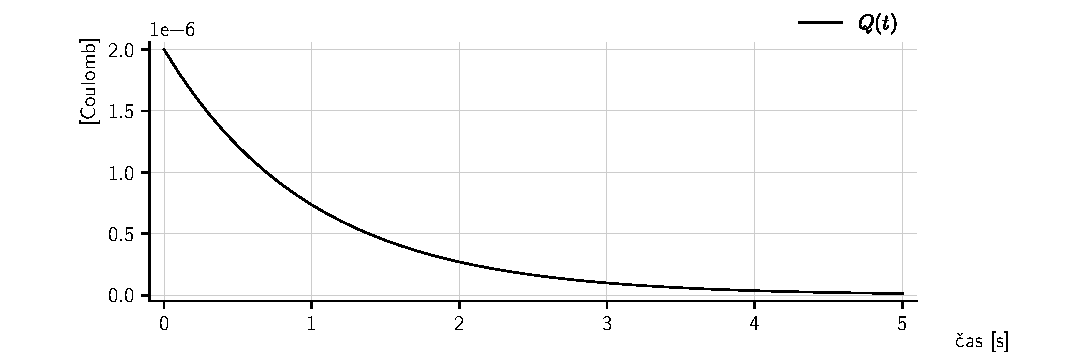
\includegraphics{../fig/cv01_fig_1.pdf}
	}

	\figcaption{Graf funkcie \eqref{rawRies2} pre $R = 10^6$ [$\Omega$], $C = 1$ [$\mu$F] a $Q_0 = 2\cdot 10^{-6}$ [Coulomb] (ľubovolné hodnoty len ako príklad)}
	\label{Graffunkcie}

    }
    
\end{center}













\subsubsection{Časový priebeh napätia na kondenzátore}


Vyšetrili sme časový priebeh elektrického náboja počas vybíjania kondenzátora. Opis situácie na začiatku časti~\ref{castVybij} však nepriamo predpokladá, že sa budeme venovať napätiu. Vzájomný vzťah už poznáme, a jeho formálne presnejší zápis (napätie $u(t)$ ako signál) je
\begin{equation} \label{QUsig}
    u(t) = \frac{1}{C} Q(t)
\end{equation}
Takže ak poznáme priebeh $Q(t)$, poznáme aj priebeh $u(t)$.

Začiatočnú podmienku pre signál $Q(t)$, teda hodnotu $Q(0)$ samozrejme tiež možno určiť so želanej (danej) začiatočnej podmienky signálu $u(t)$.
\begin{equation}
    Q(0) = C u_0
\end{equation}




\bigskip

\noindent
V zmysle úvodu časti~\ref{castVybij} uvažujme nasledujúci príklad
\begin{align*}
    C &= 1 \text{ [$\mu$F]} \\
    R &= 10^6  \text{ [$\Omega$]} \\
    u_0 &= 5  \text{ [V]}
\end{align*}
Pre tento príklad je následne začiatočná podmienka pre signál $Q(t)$
\begin{equation}
    Q(0) = 10^{-6} \cdot 5 = 0.000050 \text{ [Coulomb]}
\end{equation}
Výsledný priebeh napätia je zobrazený na obr.~\ref{PriebehNapatieDefault}.



\begin{center}
    \vbox{
        
    \makebox[\textwidth][c]{%
	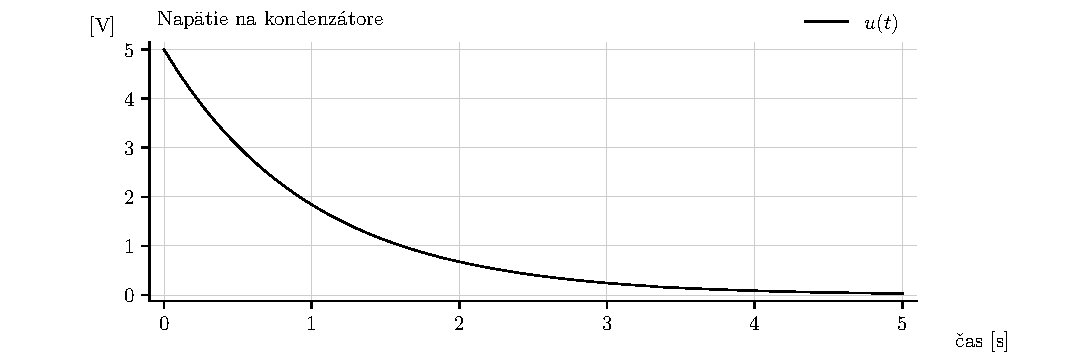
\includegraphics{../fig/cv01_fig_2.pdf}
	}

	\figcaption{Časový priebeh napätia na kondenzátore}
	\label{PriebehNapatieDefault}

    }
\end{center}









\subsubsection{Príklady pre rôzne parametre $R$ a $C$}


Pre zaujímavosť, ukážme priebeh napätia pre rôzne parametre $R$ a $C$. Príklady sú sumarizované v tabuľke~\ref{Príklady rôznych parametrov}. Graficky znázornené časové priebehy na obr.~\ref{PriebehNapatiePriklady}.



\begin{center}
    \vbox{

    \vspace{-3mm}

	\makebox[\textwidth][c]{%
	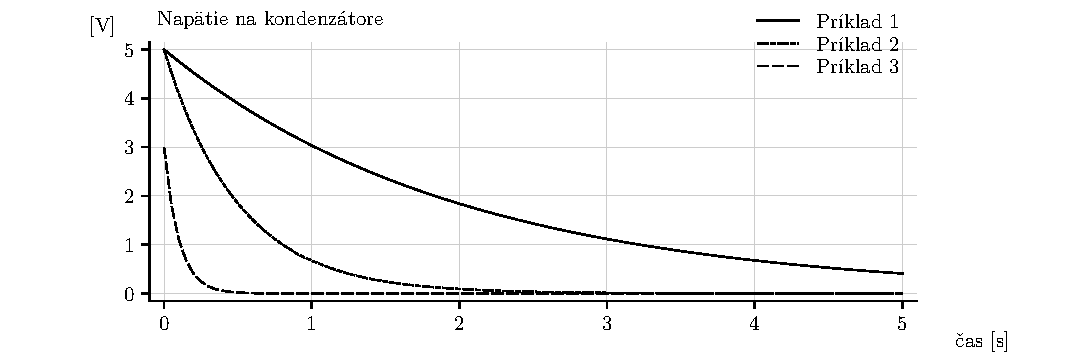
\includegraphics{../fig/cv01_fig_3.pdf}
	}

    \vspace{-3mm}

	\figcaption{Časový priebeh napätia na kondenzátore}
	\label{PriebehNapatiePriklady}

    \vspace{-3mm}

    }
\end{center}






\begin{table}[!t]
	\centering

	\caption{Príklady rôznych parametrov}
	\label{Príklady rôznych parametrov}

	\begin{tabular*}{\textwidth}{  l @{\extracolsep{\fill}} ccc }
		\toprule
            & $C$ [F] & $R$ [$\Omega$] & $u_0$ [V] \\
        \midrule
		Príklad 1 & $ 2 \cdot 10^{-6}$  & $10^{6}$  & 5 \\
		\midrule
		Príklad 2 & $\frac{1}{2} \cdot 10^{-6}$ & $10^{6}$  & 5 \\
		\midrule
		Príklad 3 &  $10^{-6}$ &  $ \frac{1}{10} \cdot 10^{6}$ & 3 \\
		\bottomrule
	\end{tabular*}
\end{table}









\section{Ďalšie poznámky}

\subsection{Vykreslenie grafu časovej funkcie -- MATLAB}

Nech cieľom je vykresliť graf časovej funkcie \eqref{rawRies2}, teda
\begin{align*}
    Q(t)   &=  Q_0 \ e^{\left( - \frac{1}{RC} t \right)}   
\end{align*}
Vzor výsledného grafu je teda na obr.~\ref{Graffunkcie}.

Takpovediac minimálny kód pre MATLAB by mohol vyzerať nasledovne:

{\catcode`\-=12
\lstinputlisting[language=Matlab,
                 caption={Súbor \lstinline{MRS01_plotexample.m}},
				 consecutivenumbers=false,
				%  linerange=c02-c02,
                 ]{../../ML/MRS01_plotexample.m}
}






\subsection{Vykreslenie grafu časovej funkcie -- Python}

Nech cieľom je vykresliť graf časovej funkcie \eqref{rawRies2}, teda
\begin{align*}
    Q(t)   &=  Q_0 \ e^{\left( - \frac{1}{RC} t \right)}   
\end{align*}
Vzor výsledného grafu je teda na obr.~\ref{Graffunkcie}.

Takpovediac minimálny kód pre jazyk Python s využitím modulov NumPy a Pyplot by mohol vyzerať nasledovne, pričom ide o bunky z jupyter notebooku:


\input{../../PY/jupynotex/tex/MRS01_plotexampleipynb_-.tex}




\bigskip

\noindent
\hrule

\medskip

\noindent
Ak sa tu čitateľ prvý krát stretáva s Python-om pre numerické výpočty, azda užitočnými mu budú tieto odkazy:

\paragraph{Python (inštalovaný ako distribúcia balíčkov...)}
Pre všeobecné používanie Python-u na Windows, obzvlášť pre „vedecké výpočty“, sa čitateľovi odporúča, tak ako sa uvádza aj tu: \url{https://www.scipy.org/install.html}, distribúcia Anaconda: \url{https://www.anaconda.com/download/}


\medskip

\noindent
Ak nie je výslovne uvedené inak, používa sa tu Python vo verzii 3.

\paragraph{Jupyter}
V týchto súvislostiach je vhodné tiež upozorniť na \url{https://jupyter.org/}. IPython ako aj Jupyter notebook sú súčasťou distribúcie Anaconda.

\medskip

\noindent
\hrule







\subsection{Numerická simulácia -- Simulink}



Ako sme uviedli, diferenciálna rovnica \eqref{diffRbeta} opisuje dynamický systém. Pripomeňme
\begin{equation} \label{diffRbeta222}
    \frac{\text{d}Q(t)}{\text{d}t} = - \frac{1}{RC} Q(t) \qquad Q(0) = Q_0
\end{equation}
kde $Q(t)$ je neznáma časová funkcia. Konštanty (nezávislé od času) $R$, $C$ a aj $Q_0$ sú známe. Úlohou je nájsť časový priebeh veličiny $Q(t)$. Nájsť riešenie diferenciálnej rovnice. V predchádzajúcom sme hľadali riešenie analyticky, výsledkom bola časová funkcia $Q(t)$, ktorej graf sme následne vykreslili.

V tejto časti budeme hľadať numerické riešenie diferenciálnej rovnice \eqref{diffRbeta222} s využitím Simulinku. Výsledkom bude časový priebeh veličiny $Q(t)$. Budú to numerické hodnoty, ktoré sú priradené k časovým údajom. Výsledok je potom tiež možné vykresliť ako závislosť $Q(t)$ od času $t$.

V simulinku je potrebné rovnicu \eqref{diffRbeta222} zadefinovať formou schematického znázornenia dynamického systému (pozri aj [\href{https://github.com/PracovnyBod/KUT/tree/main/KUT_items/KUT007/TeX}{\textsf{KUT007}}]). K tomu prislúcha nastavenie začiatočných podmienok systému (initial conditions v integrátoroch).

Pozornosť je potrebné venovať aj požadovanej časovej dĺžke simulácie, teda dĺžke časového intervalu, na ktorom požadujeme numerické riešenie dif. rovnice. Signál $Q(t)$ je možné zobraziť pomocou Scope bloku.

\begin{center}

    \vspace{-1mm}

    \makebox[\textwidth][c]{%
	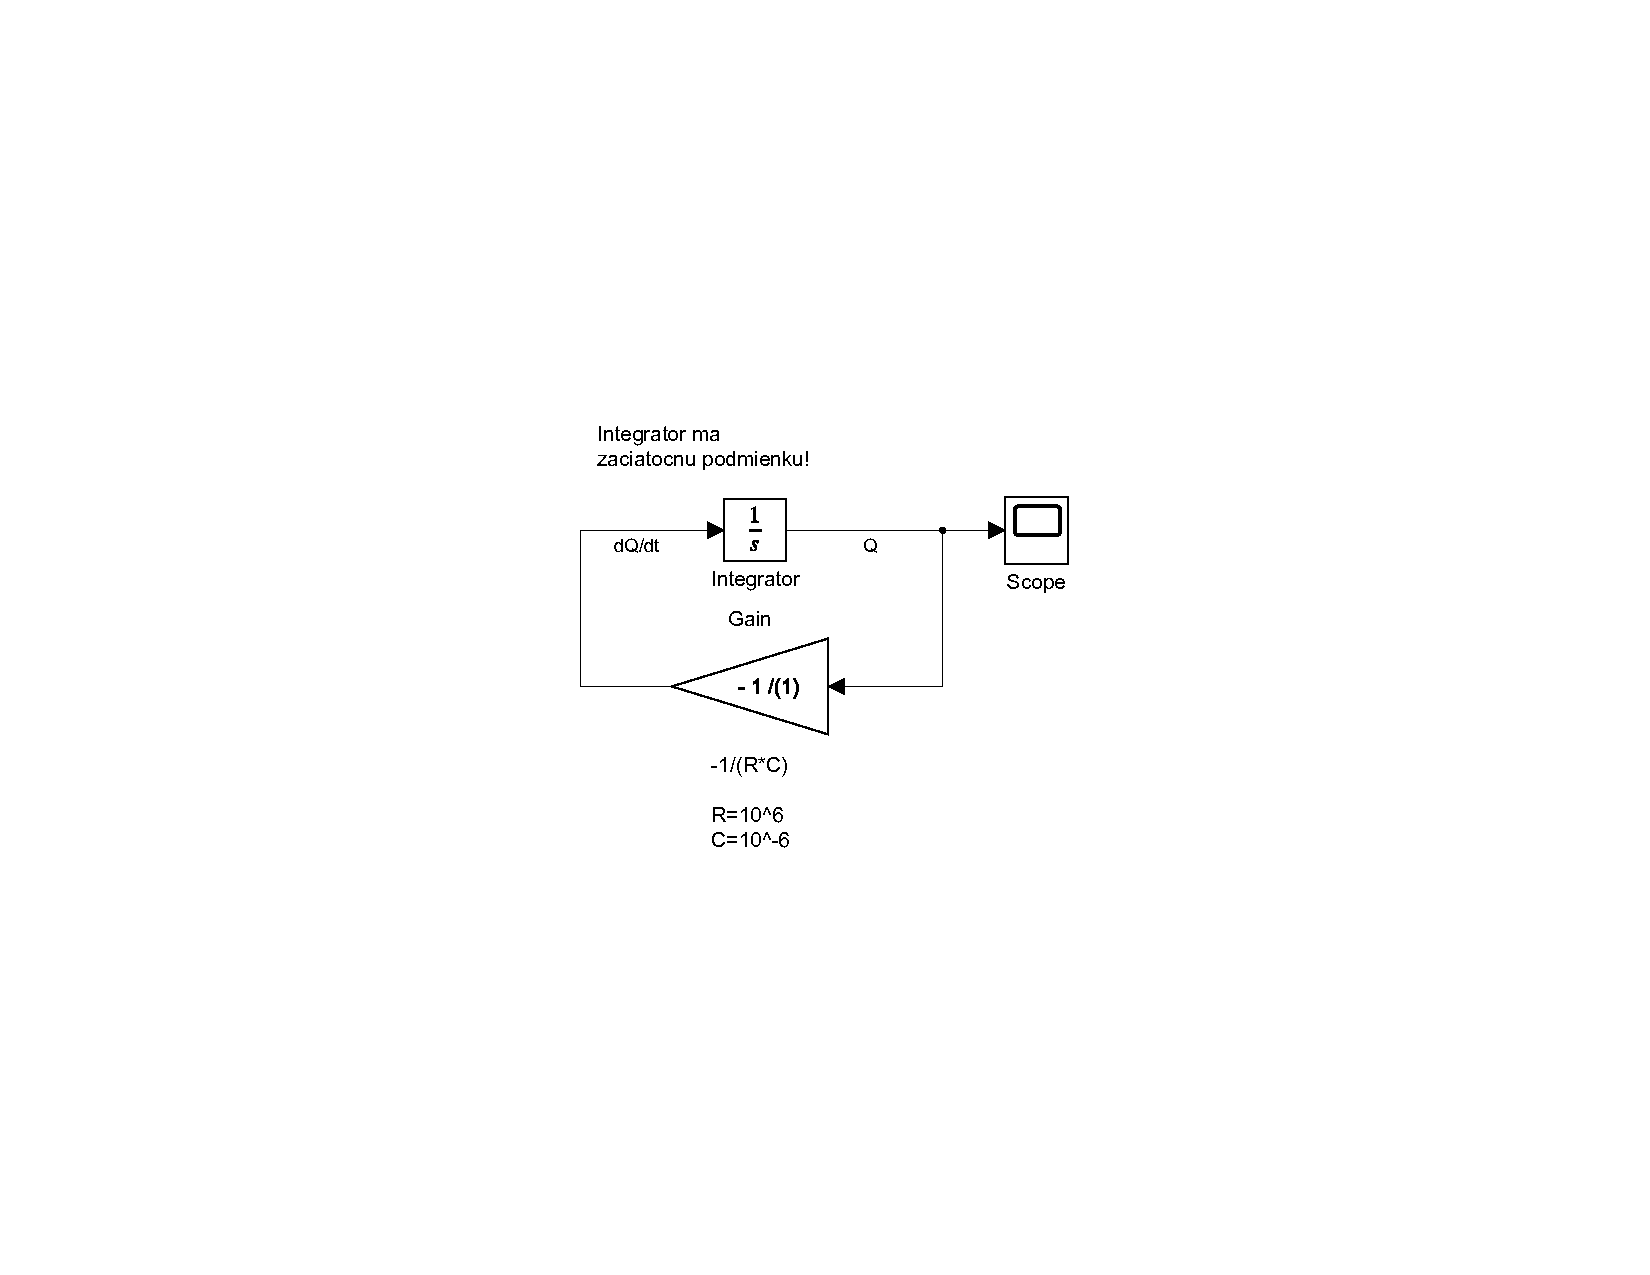
\includegraphics[trim=65mm 65mm 65mm 65mm, clip, scale=0.75]{sim_Q.pdf}
	}

    \vspace{-5mm}

	\figcaption{Simulačná schéma zodpovedajúca rovnici  \eqref{diffRbeta222}}
	\label{sim_Q}

    \vspace{-1mm}

\end{center}











\subsection{Numerická simulácia -- ODE solver (MATLAB)}



Pre numerický výpočet riešenia pomocou procedúry \verb|ode45| je potrebné predmetný systém (rovnicu) zapísať ako funkciu, ktorú bude procedúra \verb|ode45| používať. V tomto prípade:
\begin{lstlisting}[language=Matlab,]
function dQ = fundif(t,x);
R = 10^6;
C = 10^(-6);
Q = x;
dQ = -(1/(R*C)) * Q;
\end{lstlisting}
Je potrebné vytvoriť samostatný súbor \verb|fundif.m|, ktorý bude obsahovať uvedenú fuknciu, tak ako je tu uvedené.

Mimochodom, na tomto mieste nebudeme (tu v texte) uvádzať podrobnosti k~ODE solveru. Cieľom je tu len oboznámiť čitateľa s možnosťami ako získať numerické riešenie. Ako to „funguje“ bude jemne komentované neskôr.

Samotné použitie procedúry \verb|ode45| sa vykoná nasledovnými príkazmi (povedzme v~skripte v inom m-súbore):
\begin{lstlisting}[language=Matlab,]
Q_0 = 2 * 10^(-6);
[t,y] = ode45('fundif',[0 5],[Q_0]);
plot(t,y)
\end{lstlisting}
Obrázok sa ponecháva na čitateľa\ldots



\subsection{Numerická simulácia -- Python, knižnica SciPy.integrate}

Príklad použitia ODE Solvera z knižnice SciPy.integrate je možné nájsť v \lstinline|jupyter| notebooku \lstinline|PY/MRS01_ODEsolver.ipynb|.


\input{../../PY/jupynotex/tex/MRS01_ODEsolveripynb_-.tex}







\subsection{MATLAB Online Training Suite}

K uvedeným témam je možné odporučiť aj \href{https://matlabacademy.mathworks.com/online-training-subscription}{MATLAB Online Training Suite} kde základom sú kurzy:

\begin{itemize}[leftmargin=0pt, labelsep=1mm, itemsep=-4pt, topsep=0pt, ]
    \item \textsf{MATLAB Onramp} \newline {\scriptsize\url{https://matlabacademy.mathworks.com/details/matlab-onramp/gettingstarted}}
    \item \textsf{Simulink Onramp} \newline {\scriptsize\url{https://matlabacademy.mathworks.com/details/simulink-onramp/simulink}}
\end{itemize}

\noindent
Priamo k tomuto textu azda:

\begin{itemize}[leftmargin=0pt, labelsep=1mm, itemsep=-4pt, topsep=0pt, ]
    \item \textsf{Solving Ordinary Differential Equations with MATLAB} \newline {\scriptsize\url{https://matlabacademy.mathworks.com/details/solving-ordinary-differential-equations-with-matlab/odes}}
\end{itemize}













\end{document}
